\documentclass{standalone}
\usepackage[dvipsnames]{xcolor}
\usepackage{tikz}

\begin{document}
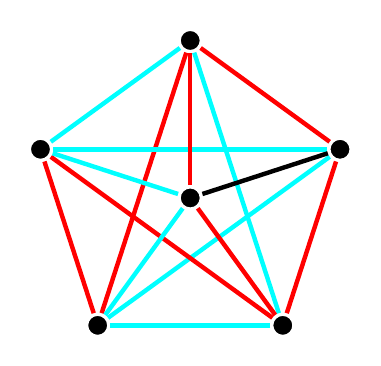
\begin{tikzpicture}

\node[draw, very thick, white, fill=black, circle, inner sep = 1mm] (n0) at (0,0) {};
\node[draw, very thick, white, fill=black, circle, inner sep = 1mm] (n1) at (90:2cm) {};
\node[draw, very thick, white, fill=black, circle, inner sep = 1mm] (n2) at (18:2cm) {};
\node[draw, very thick, white, fill=black, circle, inner sep = 1mm] (n3) at (306:2cm) {};
\node[draw, very thick, white, fill=black, circle, inner sep = 1mm] (n4) at (234:2cm) {};
\node[draw, very thick, white, fill=black, circle, inner sep = 1mm] (n5) at (162:2cm) {};

\draw[ultra thick, Red] (n1) -- (n2);
\draw[ultra thick, Red] (n2) -- (n3);
\draw[ultra thick, Cyan] (n3) -- (n4);
\draw[ultra thick, Red] (n4) -- (n5);
\draw[ultra thick, Cyan] (n5) -- (n1);

\draw[ultra thick, Cyan] (n1) -- (n3);
\draw[ultra thick, Cyan] (n2) -- (n4);
\draw[ultra thick, Red] (n3) -- (n5);
\draw[ultra thick, Red] (n4) -- (n1);
\draw[ultra thick, Cyan] (n5) -- (n2);

\draw[ultra thick, Red] (n1) -- (n0);
\draw[ultra thick, black] (n2) -- (n0);
\draw[ultra thick, Red] (n3) -- (n0);
\draw[ultra thick, Cyan] (n4) -- (n0);
\draw[ultra thick, Cyan] (n5) -- (n0);



\end{tikzpicture}
\end{document}